\documentclass[11pt]{article}
\usepackage{amsmath,amssymb,float,amsfonts,enumitem,tcolorbox}

\include{macros}


\title{Project 1 Redwood Data Report}
\author{Phoebe Abramowitz(26386343) & Omri Newman(3032273024)}
\date{Due by: \textbf{11 PM, Friday, Mar 8}}

\usepackage{Sweave}
\begin{document}
\Sconcordance{concordance:project1writeup.tex:project1writeup.Rnw:%
1 4 1 1 11 5 1 1 0 21 1 1 33 2 14 8 1 1 14 1 18 3 1 1 3 7 0 1 1 5 0 1 1 %
5 0 1 1 5 0 1 3 2 0 1 2 6 0 1 3 5 0 1 2 2 1 1 13 36 1}


\maketitle

\section{Paper Summary (20 pts)}

\item This study of microclimatic monitoring aims to get a better understanding of the life of a Redwood tree in Sonoma, CA. To do this, an interdisciplinary team from the University of California, Berkeley designed an experiment that paints a picture of a redwood tree’s ecophysiology spanning fourty-four days in Spring 2004. They did this using a unique network of nodes and wireless sensors to gather spatio-temporal and environmental dynamic data over the entire organism. Each of the thirty-three nodes collected hundreds of thousands of data points, which lie in four different three-dimensional spaces (time x height x value). This wireless sensor network, or macroscope, allows for rich analysis on an unprecedented dataset.
After brainstorming with several biologists, Sonoma’s coastal redwood forest was chosen as the site of this study because of its dynamic ecosystem. Longer daylight hours during the Spring provided sufficient time for the photosynthetically active radiation sensors to collect data, and the coastal fog coming off the Pacific guaranteed a wide range of temperature and humidity gradients.
A thorough analysis of the redwood data confirmed the biologists’ hypothesis, which premised the existence of dynamic gradients present in the redwood trees ecophysiology. By projecting the data points onto a subset of the three-dimensions, the analysis task became simpler.
 One drawback to using the sensor network was the presence of missing values throughout the data set in both time and height dimensions. However, the team worked in spite of this by studying distributions in most of their analyses.  In addition to confirming the team’s hypothesis, more information about the climatic distribution of the tree was extracted from the analysis. One impactful step was using the data to build a quantitative model of the effect of microclimatic gradients on the sap flow rate of redwood trees. By better understanding this process, biologists can piece together a more detailed picture of the larger scale carbon and water exchange within a forest ecosystem.
The main variables of interest in this study are those that shed light on the microclimate and ecophysiology of the redwood tree. Thus, each data point can be viewed in three dimensions-- time, height, and value. The values, recorded by the network of sensors, are temperature, humidity, incident photosynthetically active solar radiation (PAR), and reflected PAR. Collecting this data over an extended period of time required a powerful system and precise deployment methodology. The data collection time period started in late April and spanned fourty-four days, sampling all sensors every five minutes. The nodes were placed along the seventy meter redwood tree starting at a height of fifteen meters, with two-meter spacing between nodes. The west side of the tree had a thicker canopy that served as protection against environmental effects, so the majority of the nodes were placed there. Lastly, the nodes were placed close to the trunk (0.1-1.0 meter) such that the recordings were of the microclimatic trends of the tree and not the wider climate.
Multiple sensors were integrated into the Mica2Dot wireless node, as a means to gather data on the environmental dynamics of the tree. This node has a one inch diameter form factor, an Atmel microcontroller running at 4 MHz, a 433 MHz radio from Chipcon operating at 40Kbps, and 512kB of flash memory. The node was packaged into a sealed cylindrical enclosure made from white high-density polyethylene that reflects radiated heat. The enclosure contained the node, battery, and two sensor boards - one for direct radiation and one for all other measurements. Data collected from these nodes were stored in a local database or gateway, then transmitted to an offsite database via a general packet radio service (GPRS) cellular modem. The UCB team used TASK software as the node operating system and data collection scheme to aid with this work. This multi-hop system utilized TinyOS and MintRoute systems to retrieve data from the nodes and store them in the gateway as efficiently as possible. The entire network of nodes was awake for four seconds every five minutes, in order to take sensor readings, transfer the data to the base stations, and then return to sleep.
Two calibration schemes were completed by the team to ensure a satisfactory operation prior to setting up the final system. The first calibration consisted of leaving the sensors on a roof collecting PAR data every thirty second for two weeks to verify the accuracy of the readings. The purpose of the second calibration was to understand the response of the temperature and humidity sensors. The nodes were tested in a controllable weather chamber that had varying temperature and humidity conditions, and recorded readings every thirty seconds. The calibration techniques used on the nodes took up space on the 512kB flash memory. Thus, some of the data loggers in the local database gateway ran out of memory before the end of the data collection time period. These loggers were meant to serve as a backup in case of network failure, and stored data in the case of lost GPRS connectivity. On the other hand, the logger data that was stored in the gateway could only be accessed at the end of the data collection time period, and there was lost information in the nodes that ran out of flash memory. This defines the main difference between sonoma-data-net.csv and sonoma-data-log.csv, which both contain values the other is missing.

\section{Data cleaning (40 pts)}

This data set contains gross outliers, inconsistencies, and lots of missing values. We use basic exploratory data analysis and data cleaning techniques to get a better understanding of the data, determine which values make sense in the context of the study, and remove missing values when necessary.

\begin{enumerate}[label=(\alph*)]
\item
For the initial comparison in hamatop (Incident PAR) between \textbf{sonoma-data-log.csv} and \textbf{sonoma-data-net.csv}, we remove outliers that are ten times larger than the third quartile in an effort to explore the ranges more thoroughly. We notice a slight bump in the right tail of incident PARs histogram for \textbf{sonoma-data-net.csv}, which does not occur in \textbf{sonoma-data-log.csv}.
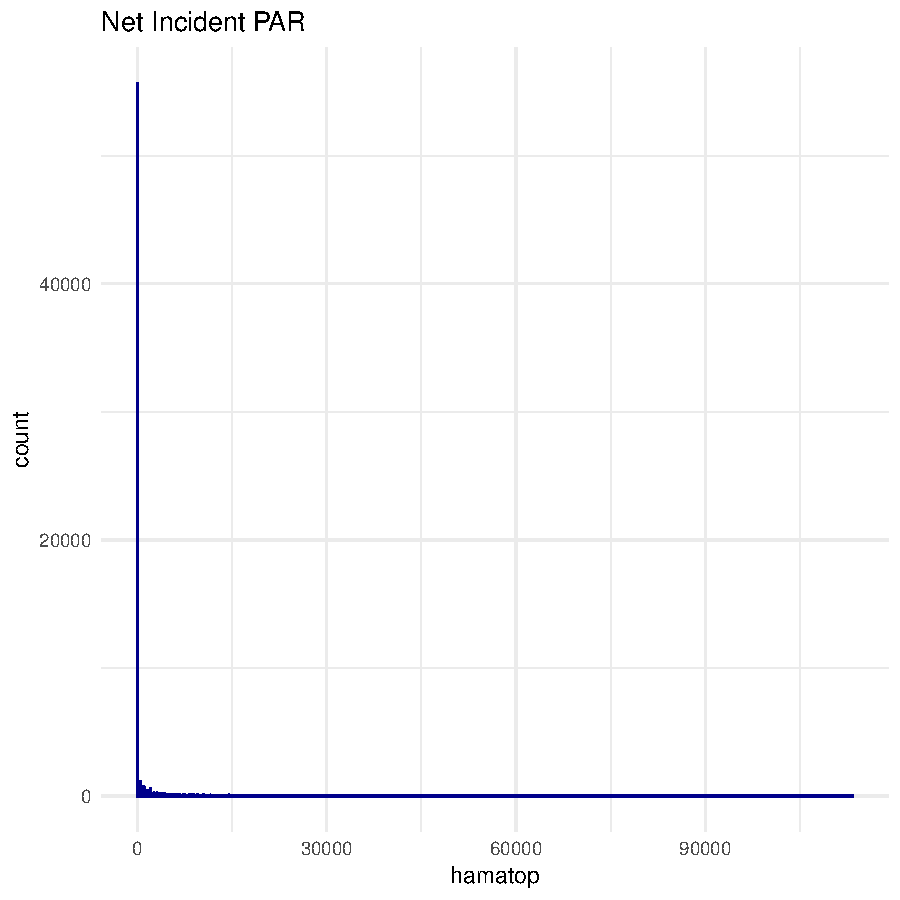
\includegraphics{project1writeup-002}
The histograms for hamabot (Reflected PAR) reveal some interesting trends that both \textbf{sonoma-data-log.csv} and \textbf{sonoma-data-net.csv} share. Not only are the ranges the same between the two, but they both exhibit the same gaps in the data.
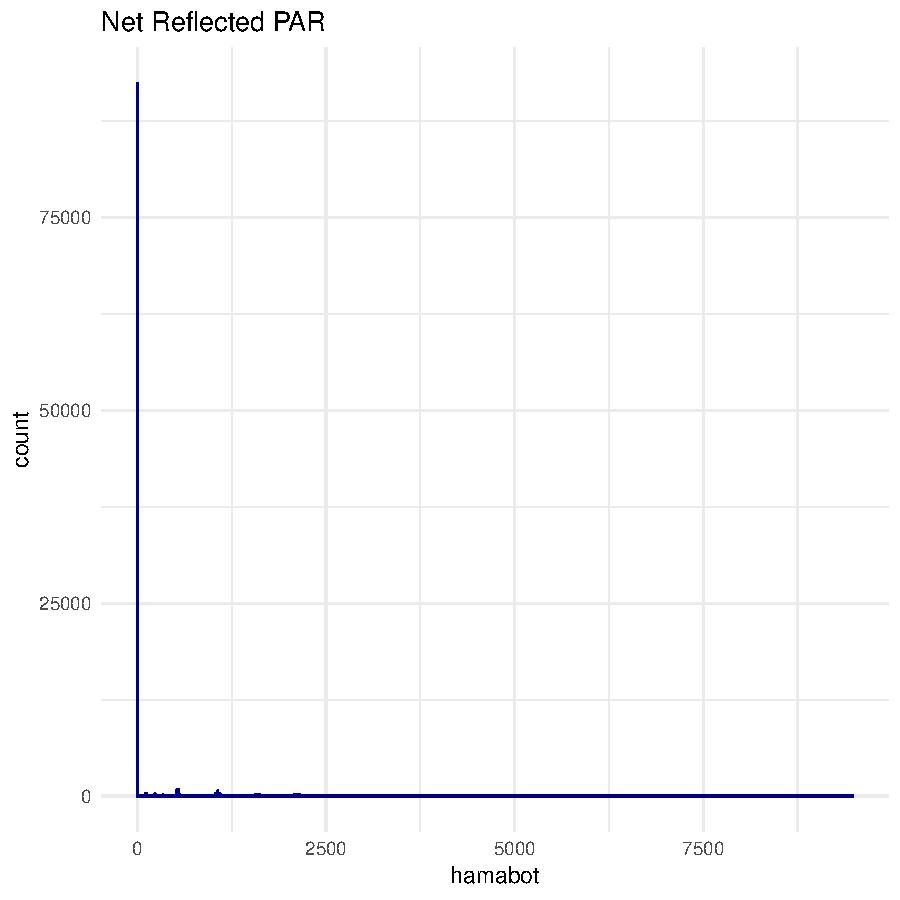
\includegraphics{project1writeup-003}
It is clear from the histograms below that voltage readings are not consistent between \textbf{sonoma-data-log.csv} and \textbf{sonoma-data-net.csv}.
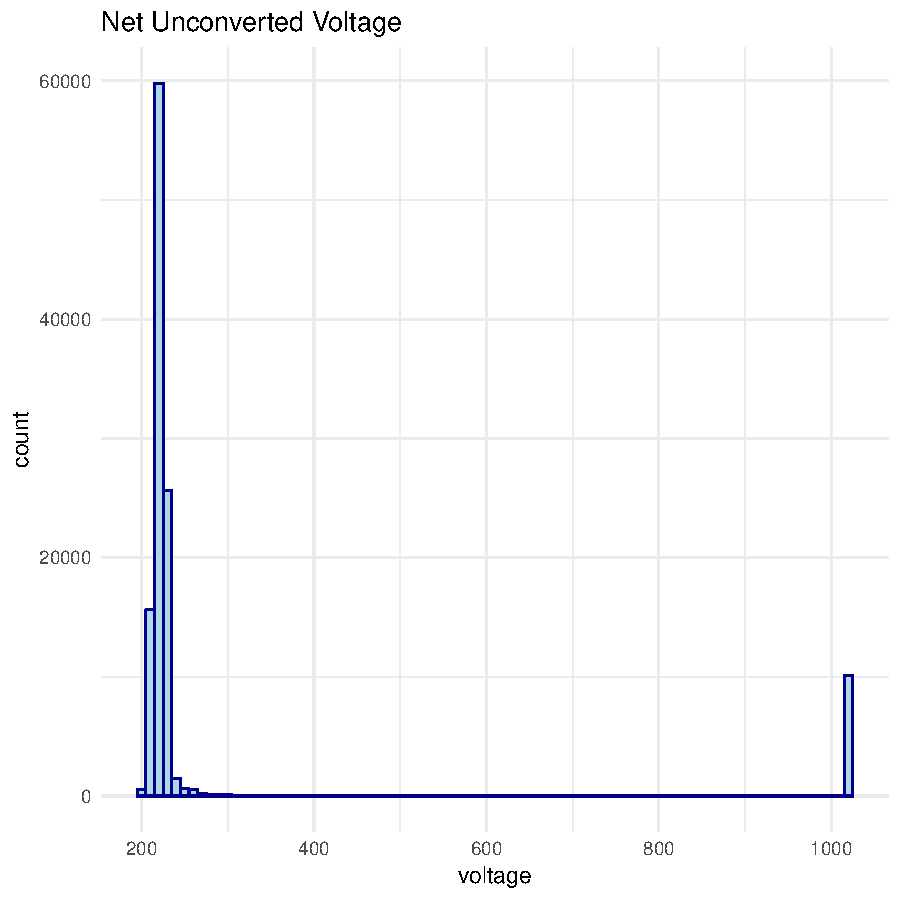
\includegraphics{project1writeup-004}

To reconcile the inconsistencies between voltage and PAR, we applied two separate conversions as to match the ranges from the paper: \newline
The voltage readings in \textbf{sonoma-data-log.csv} are all within the correct range of just a few volts, while the readings in \textbf{sonoma-data-net.csv} had significantly higher values. This discrepancy can be attributed to the analog-to-digital converter used within the ATmega128 node $^1$. To switch from the 10-bit ADC readings to actual voltage measured, we followed a simple ratiometric conversion scheme $^2$. We multiplied the values by 12.33 and divided by 1023 which transformed the data into the desired range.

We also noticed the ranges for hamatop and hamabot differ from the paper. We convert the measurements of both types of PAR from Lux to PPMG, the units expressed in the visualizations in the study which requires a 0.0185 conversion factor.


While they are not shown here, the histograms of temperature and humidity revealed no inconsistencies in the ranges, only some outliers.

\begin{Schunk}
\begin{Sinput}
> # ONLY RUN THIS ONCE!!!
> # Converting data to same range
> 
> #Incident and Reflected PAR
> data_net$hamatop <- data_net$hamatop*0.0185
> data_net$hamabot <- data_net$hamabot*0.0185
> data_log$hamatop <- data_log$hamatop*0.0185
> data_log$hamabot <- data_log$hamabot*0.0185
> # Voltage
> data_net$voltage = data_net$voltage*12.33 / 1023
\end{Sinput}
\end{Schunk}

\begin{Schunk}
\begin{Sinput}
> # Concatenate everything in data_net with everything in data_log
> # that isn't in data_net, defined by epoch and nodeid
> just_log <- anti_join(data_log, data_net, by = c("nodeid" = "nodeid", "epoch" = "epoch"))
> all_readings <- full_join(data_net, just_log)
> # to combat different error all_readings <- all_readings[,1:11]
> 
> # Cleaning all_readings before adding mote_location
> df <- all_readings %>%
+   select(c("result_time", "epoch", "nodeid", "voltage", "humid_temp", "humid_adj", "hamatop", "hamabot")) %>%
+   rename(temp = humid_temp) %>%
+   rename(humid = humid_adj) %>%
+   rename(incident_PAR = hamatop) %>%
+   rename(reflect_PAR = hamabot) %>%
+   mutate(result_time = as.POSIXct(result_time))
> 
\end{Sinput}
\end{Schunk}

\item
In our main data table, we remove 3686 rows where the temperature, humidity, reflective PAR, and incident PAR are missing. There are 3686 values missing for each of the 4 variables.
\begin{Schunk}
\begin{Sinput}
> #Number of missing values for each variable(don't display this)
> sum(is.na(df$temp))
\end{Sinput}
\begin{Soutput}
[1] 4262
\end{Soutput}
\begin{Sinput}
> sum(is.na(df$humid))
\end{Sinput}
\begin{Soutput}
[1] 4262
\end{Soutput}
\begin{Sinput}
> sum(is.na(df$incident_PAR))
\end{Sinput}
\begin{Soutput}
[1] 4262
\end{Soutput}
\begin{Sinput}
> sum(is.na(df$reflect_PAR))
\end{Sinput}
\begin{Soutput}
[1] 4262
\end{Soutput}
\begin{Sinput}
> #Initial Number of rows missing any measurements
> na_vals <- df %>% filter(is.na(temp)) %>% filter(is.na(humid)) %>%
+   filter(is.na(incident_PAR)) %>% filter(is.na(reflect_PAR))
> #we dont want it to evaluate this value
> nrow(na_vals)
\end{Sinput}
\begin{Soutput}
[1] 4262
\end{Soutput}
\begin{Sinput}
> #Remove missing Data rows
> df <- df %>% filter(!is.na(temp)) %>% filter(!is.na(humid)) %>%
+   filter(!is.na(incident_PAR)) %>% filter(!is.na(reflect_PAR))
\end{Sinput}
\end{Schunk}

\item
After removing missing data, reconciling inconsistencies, and joining the \textbf{sonoma-data-log.csv} and \textbf{sonoma-data-net.csv}, we incorporate the \textbf{mote-location-data.txt} using nodeid as a unique identifier. All together we have the location of each mote within the two trees, along with the respective sensor data. We selected only the variables of interest amongst the 11 to create a desired dataset of all the readings. Our main table has 337,744 observations and 12 variables.
\begin{Schunk}
\begin{Sinput}
> # Incorporate mote_location into all_readings
> mote_location <- mote_location %>%
+   rename(nodeid = ID)
> main <- left_join(df, mote_location) %>%
+   rename(height = Height) %>%
+   rename(direc = Direc) %>%
+   rename(dist = Dist) %>%
+   rename(tree = Tree)
> 
> #337743 observations of 12 variables
\end{Sinput}
\end{Schunk}

\item
We worked to match the range of each variable as they are presented in the paper. It is clear in the following histograms that all of the variables contain some outliers. Instead of removing these data points per variable, we noticed that filtering out faulty voltage readings does the same job in one fell swoop. Just as is described in the paper, filtering out readings below 2.4V or above 3V removes 33,833 observations.
\begin{Schunk}
\begin{Soutput}
   Min. 1st Qu.  Median    Mean 3rd Qu.    Max. 
  0.000   0.000   0.000   3.529   0.000 175.394 
\end{Soutput}
\begin{Soutput}
   Min. 1st Qu.  Median    Mean 3rd Qu.    Max. 
   0.00    0.00    0.00  135.65   96.67 2097.46 
\end{Soutput}
\end{Schunk}
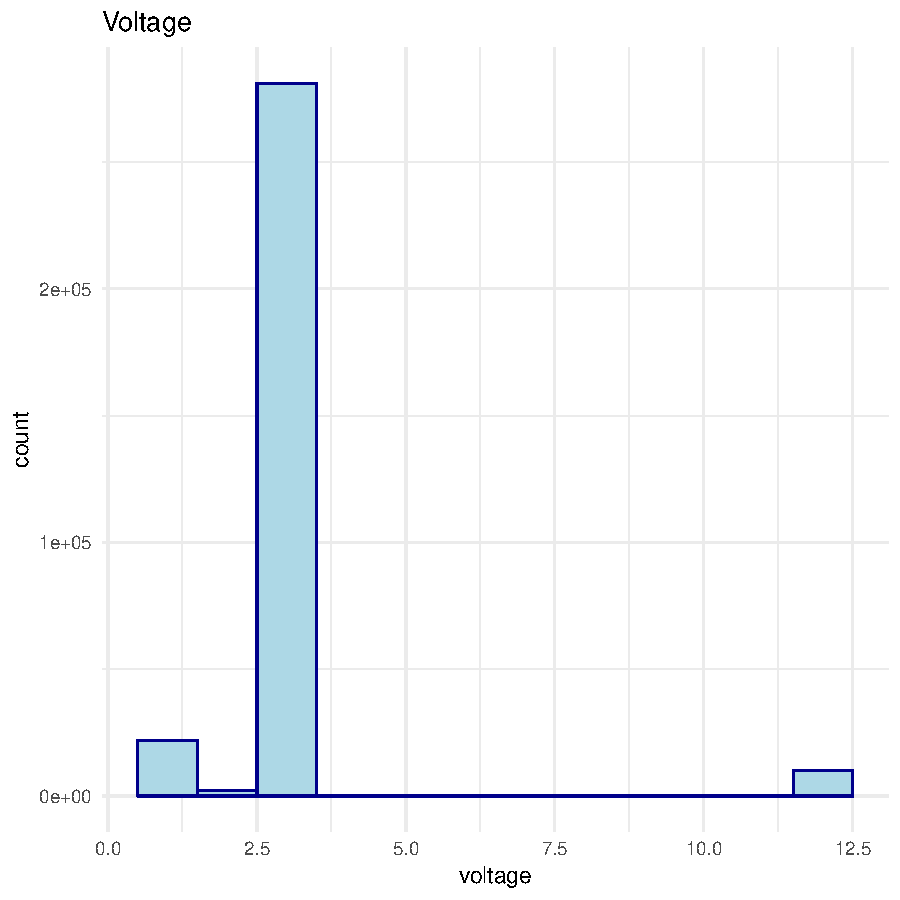
\includegraphics{project1writeup-009}

